% 背景\cite{lecun2015deep}

\section{绪论}
 
\subsection{背景}
% 思路: ​
% 企业从封闭式组织转变为开放式组织。理由(原因):
%       有互联网技术提供基础保障
%       变迁的生产方式推动企业管理模式的变化
% 开源社区是一种典型的开放式组织形式。
%       传统软件开发方式与开源软件开发的区别​
%       开源蓬勃发展
% 开源社区/开放式组织需要治理
% //TODO: 引用能否直接引原文?还是说简述一个观点并标明出处?
\par 随着互联网技术的发展,越来越多的企业开始逐渐从传统的封闭式组织转变为开放式组织。传统的自上而下、封闭式、命令式与控制式的组织管理方式正在走向终结,而开放透明、高效敏捷的开放式组织管理方式正在成为新的潮流。一方面,互联网技术为开放访问、开放协议以及开放协作的文化提供了基础保障。技术的发展使得全世界的知识型人才能够通过互联网进行沟通和交流,并使得他们能够平等和自由的相互分享和贡献自己的盈余资源,如想法、创意以及才智等。大家在自发交互沟通中达成共识并创造出群体智慧,产生了如维基百科、开源软件开发平台(如GitHub)等创新型产品和服务\cite{王璐2017开放式创新的协同演化机制研究}。 另一方面,全球经济数字化浪潮正蓬勃发展,以移动通信、物联网、人工智能等为代表的新一代信息技术将人-业务-系统-组织-企业连接成一个网络,传统的业务系统从一个简单的机械系统演变成一个复杂的生态系统,企业在从局部优化走向全局优化的过程中,不断变迁的生产方式推动着企业管理模式的变化,而这些变化都驱动着企业组织不断被重构与再定义。

\par 近些年来,开源作为一种典型的开放式组织管理形式,在软件开发领域发挥了巨大作用,推动了现有的生产方式的变革。长期以来,产品、项目形式的专有软件开发是软件生产的主流,其特点是精英化(专业骨干制作软件)、计划性(预先规划需求/自顶向下开发)、封闭性(开发过程不对外开放)、许可证(商业模式通过销售软件产品获利)。这种软件生产方式的问题在于开发成本过高、开发周期较长、补丁漏洞防不胜防。与之相反,幵源软件的开发者通过一种开放的软件许可协议保护其著作权,其源代码、设计文档、幵发日志等数据允许用户自由的学习、修改和传播。开源软件的开发模式不仅是一种依托开放、开源的软件合作社群而且正向基于分享、交互与群体智能的同侪生产方式发展,其特点是开发过程从封闭到开放、开发人员从精英到大众、开发组织从工厂到社群、开发成果从产品到服务。在此方式下,使用者与设计者、开发者、维护者之间不再壁垒森严,维基百科等己证明了这种生产方式对于知识型制品的优越性。\cite{李其锋2014面向开源社区的开发者群体行为分析方法}

\par 开源软件经过了 20 多年的发展,已经演化出诸如 Linux、MySQL、Hadoop、Kubernetes、TensorFlow、React、VS Code 这些数字化的基础设施,而且整个技术栈还在不断向上生长,吞噬着整个软件世界,并形成了一个开源生态,一个开源文明。由代码、数据、开发者行为、社区规范等等所组成的开源数字生态系统,就像一个新物种一样,不断演化与成长,支持着整个数字世界的基础设施,也在逐渐改变人类的协作与行为方式。开源协作平台也将成为一个海量数据市场,在这个市场里,将有大量透明化的信息,同时拥有做出决策和进行协作的数字工具。这一切将产生巨大的影响,不只是对组织和管理者,而且对所有生态中的各类参与者,包括开发者、社区经理、工程师、还有消费者。

\par 开源软件开发者分布在全球不同位置,进行相对独立的软件开发,开发者的立项、讨论、评价、修改、测试等行为,主要是通过互联网相互沟通、讨论和协商实现。开源软件开发过程中的交互方式不同于基于企业内部层级式组织的专有软件开发,而是依靠自组织、分布式的开源社区,通过项目发起者协调,这就导致质量、成本这些因素成为在软件开发过程中受交互行为影响的外生变量,而不同于专有软件的厂商自己决定的内生变量。\cite{李其锋2014面向开源社区的开发者群体行为分析方法}因此,开源需要有一整套的治理框架,基于此框架的数字化、自动化的治理工具来帮助开源项目及社区更高效的运作和管理。

\par 开源的本质是开放式组织管理。开放式组织中的人员以兴趣爱好聚集,可快速地加入和退出,人员流动较快。但却不能缺少传统企业运营中的每一个环节,例如人员招聘、项目管理、人力绩效、工资分红、退出机制、宣传营销等。因此,开放式组织需要有一套治理框架。框架中包含有松耦合的进入与退出机制、完善的数字化管理监控体系,从宣传、活动、用户、开发、管理、布道等各个方面进行数字化管理和常态化的社区角色快速转换,并有完善的自动化机制保证社区角色快速转换中足够低的学习成本和转换成本。

\par 本课题正是致力于完善开源社区中的数字化治理框架,结合机器人流程自动化的形式,实现一个浏览器插件的看板应用,协助开源社区中不同项目、不同视角的决策与运营。


\subsection{相关工作}
% 思路: Hypertrons 项目现状
\par 为了完善开源社区的架构、更好地治理开源社区,使其成为如今商业社会中更具价值的数字化生产社区,开源开发者们在社区治理方面做了许多工作,他们的力量回馈到开源社区,成为了新的发展方向。这其中,最显著的变化便是Github Apps自2016年推出以来的迅猛发展。

\par Github Apps也称为自动协作机器人,它们本身是Github的独立账号,用户名以[bot]结尾,在开源社区中拥有独立的认证身份;但其实它们本质上是一种程序,能够自动化地帮助用户使用 Github 提供的认证信息、调用 Github API来完成一系列相对复杂的操作,如检查代码合并、签署许可协议等,以减少重复的人工劳作。GitHub Apps的优点有很多,一个比较突出的优势是,GitHub Apps可以做到对权限的精细管理,比如负责持续集成的GitHub Apps可以请求对仓库内容的读取权限和对状态的写入权限,又比如一个GitHub Apps可能没有对代码的读取或写入权限,但仍能管理issues、labels和milestones。

\par 在目前Github平台全球最活跃开发者账号中,大部分为GitHub Apps。据多年的数据统计,GitHub Apps年活跃账号数量(活跃数量)与所产生日志总量占全年日志占比(日志占比)的变化如图1.2所示:从日志占比来看,2019年相较于2018年提升了288\%,2020年相较2019年增长141\%,达到了12\% 以上。总体而言,Github Apps的流行趋势不可遏制,这也侧面反映着开源社区的发展进程对Github Apps这一类智能化治理的功能需求日益增加。
\begin{figure}[H]
    \centering
    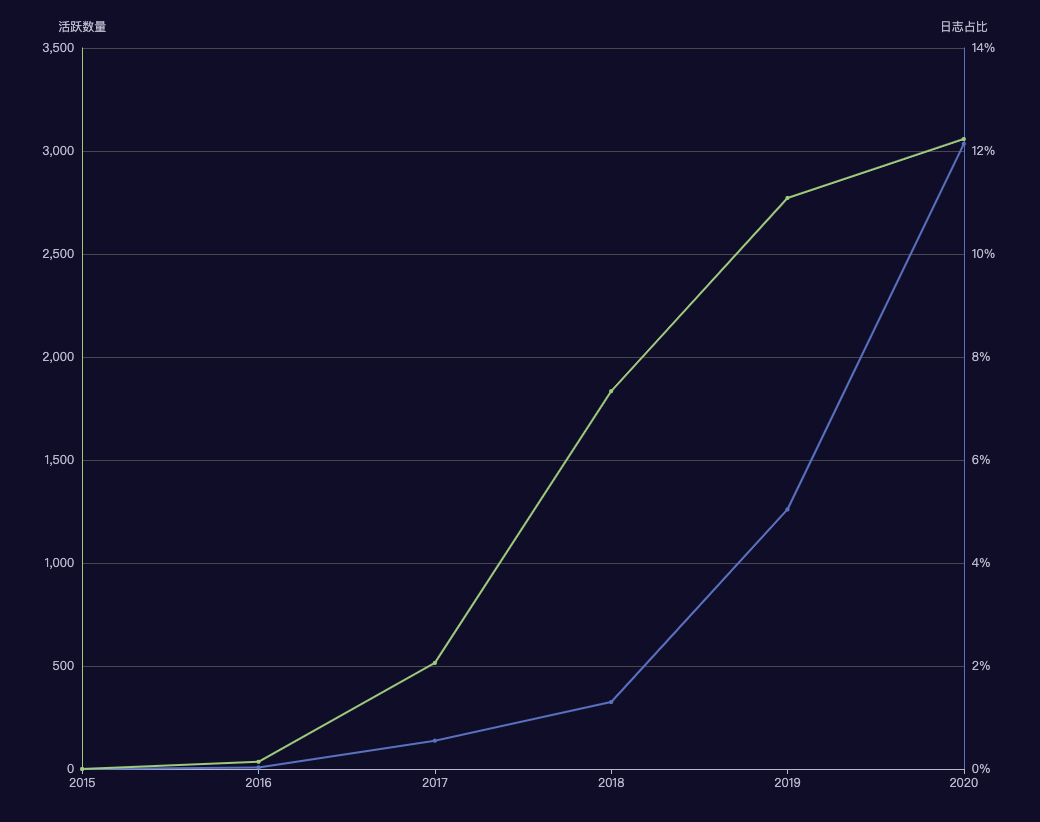
\includegraphics[width=130mm]{./figures/image1-2.png}
    \caption{GitHub Apps活跃账号数量与日志占比\\Figure 1-1: The number of GitHub Apps active accounts and the proportion of logs}
\end{figure}

\par 在这样的大环境之下,由华东师范大学与同济大学跨校组建的实验室X-lab设计并发起了一个面向开源项目的RPA(Robotic Process Automation机器人流程自动化)平台——Hypertrons,致力于向开源代码平台提供流程自动化定制与运行的能力。在开源社区中,Hypertrons扮演着开源项目和开放组织中的一个智能的数字劳工的角色,承担一些流程的自动的构建与编排,为跨平台的组织管理工作提供便利。在功能上,它依托于对全域开源行为的开放数据分析结果,帮助开发者与社区管理者进行决策,其方式是提供一个高度可配、高度可移植的框架,供用户在项目级别自定义组件,以配合不同项目的管理流程与制度。在开发者通常使用的各个平台(如Git、Gitlab、Github、Gitee、Slack、Jenkins、邮件、石墨文档和各类线上服务)之间,Hypertrons提供了跨平台交互的能力,同时为了更好地做出决策,也采集各平台的开放数据作为决策基础,为社区的数字化运营分析提供了有效的支撑。

\par 在Hypertrons项目中,不论是在项目层面对于用户行为数据的采集,还是将数据分析结果呈现给用户,都是一个无法避免地与用户产生联结、进行交互的过程。于是,为了更好地以交互的方式展现Hypertrons社区的数字化运营分析结果、辅助用户决策,面向开放组织的迷你看板项目应运而生。由于不希望深度改变用户的使用习惯,故发起一个浏览器插件项目,通过在特定网址的网页中插入迷你看板的方式为开放组织提供有效的监控和运营手段,这个项目是Hypertrons一大创新,也是Hypertrons的前端展示模块与功能延伸,即重要的组成部分。


\subsection{拟解决的主要问题}
% 思路:
% Hypertrons 没能做到的事情(或hypertrons与本项目的关系)

\par 一方面,迷你项目看板作为Hypertrons在浏览器端的入口之一,是Hypertrons的多平台集成与扩展能力的展示与增强。另一方面,通过该项目,可以非常方便且低成本地进行精细化市场运营:掌握用户的行为数据和兴趣偏好等重要信息,从而针对不同用户进行个性化的数字运营。

\par 经调研,在目前的各大代码托管平台中,仅项目页面会显示一些低阶指标数据(如Star数、贡献者列表等)与有限的的高阶指标数据(如GitHub Insights页面)。使用这些平台自带的功能,用户无从了解更多的高阶数据指标(如项目活跃度、流行度、贡献者活跃度、Issue平均响应时间等),从而无法很好或快速地掌握项目状况,进行管理或协同工作。而市面上已有的同类型看板应用,虽然也有用于项目健康度衡量分析的指标,但它们都以独立部署的平台、网站的形式呈现,无法很好地在此场景下为不同角色、不同平台的用户服务。于是,以浏览器插件形式存在的迷你看板成为了该场景下的一种更优解。

\par 根据Hypertrons的需求与迷你项目看板的产生动机,本课题关注的主要问题有两个:一是如何将开源社区中的开放数据进行分析呈现,即,可视化给用户;二是提供一种简单易用的交互方法,接收用户管理与配置的定制化指令(也即用户行为数据)。

\subsection{论文组织}

\par 本文在第一章介绍了课题的相关背景与产生动机,对应地提出拟解决的主要问题;在第二章中,将展开讲述如何对开源社区中的开放数据进行分析,包括了从数据的获取、探索性分析到数据预处理的流程;接下来的第三章,会根据前面分析得到的指向性信息,对不同业务场景开展数据设计;而第四章则从技术的角度,详述了面向开放组织的迷你看板应用的整体实现细节。